\section{Exact preservation of monthly marginals}
\label{app:marginals}

\begin{proposition}
For any target window, calendar month, resource, and resampled member, the rank reassignment preserves the complete empirical marginal distribution of the corrected values.
\end{proposition}

\begin{proof}
Fix a calendar month and resource. Let $I$ denote the set of its $n$ day indices across the target window, and let $c_{(1)}\leq\cdots\leq c_{(n)}$ be the ordered corrected values on $I$. The stable sort of the resampled scores yields an ordering $\pi_1,\ldots,\pi_n$ of the same date indices. The output assigns $c'_{\pi_j}=c_{(j)}$ for each $j$. Because each index occurs once in this assignment, for every real $u$,
\[
\frac{1}{n}\sum_{t\in I}\mathbf{1}\{c'_t\leq u\}
=\frac{1}{n}\sum_{j=1}^{n}\mathbf{1}\{c_{(j)}\leq u\}
=\frac{1}{n}\sum_{t\in I}\mathbf{1}\{c_t\leq u\}.
\]
Both empirical distribution functions agree pointwise. Repeated corrected values and score ties satisfy the same equality because the stable ordering assigns every value with its original multiplicity. The assignment acts separately on each variable, so equality of the individual distributions leaves room for changes in same-day pairs and multi-day runs.
\end{proof}

\section{Dispatch mass balance and tank capacity}
\label{app:dispatch}

\begin{proposition}
The daily rule in Eq.~\eqref{eq:dispatch} conserves hydrogen when surplus discarded at full capacity is included. For the same production sequence and warm-up, daily unmet delivery is weakly decreasing with tank capacity.
\end{proposition}

\begin{proof}
Let $K=kD$ be tank capacity and write discarded surplus as $W_t=\max\{B_t-K,0\}$. The identity
\[
\clip(B_t,0,K)=B_t+\max\{-B_t,0\}-\max\{B_t-K,0\}
\]
follows by considering $B_t<0$, $0\leq B_t\leq K$, and $B_t>K$. Substituting $B_t=S_{t-1}+G_t-D$ and $U_t=\max\{-B_t,0\}$ gives
\[
S_{t-1}+G_t=(D-U_t)+S_t+W_t.
\]
The terms on the right are delivered mass, closing inventory, and discarded surplus. For capacities $K_1\leq K_2$, both inventories start at zero before warm-up. If $S_{t-1}^{(1)}\leq S_{t-1}^{(2)}$ then $B_t^{(1)}\leq B_t^{(2)}$ for the common production and demand. The function $\clip(B,0,K)=\min\{K,\max\{B,0\}\}$ is nondecreasing in both arguments. Thus $S_t^{(1)}\leq S_t^{(2)}$ and $U_t^{(1)}\geq U_t^{(2)}$. Induction through warm-up and the scored dates proves the result. Summing over a year preserves the inequality for annual unmet demand.
\end{proof}

\section{Sorted expression for empirical CRPS}
\label{app:crps}

\begin{proposition}
For the list of simulated losses sorted as $z_{(1)}\leq\cdots\leq z_{(M)}$, the spread term of Eq.~\eqref{eq:crps} equals
\[
\frac{1}{2M^2}\sum_{i,j=1}^{M}|z_i-z_j|
=\frac{1}{M^2}\sum_{k=1}^{M}(2k-M-1)z_{(k)}.
\]
\end{proposition}

\begin{proof}
The double sum is invariant to sorting. Its diagonal terms vanish, and the strict upper and lower triangles have equal sums. For each $i<j$, the absolute difference is $z_{(j)}-z_{(i)}$. Hence
\[
\tfrac12\sum_{i,j=1}^M |z_i-z_j|
=\sum_{i<j}(z_{(j)}-z_{(i)})
=\sum_{k=1}^{M}\bigl((k-1)-(M-k)\bigr)z_{(k)}.
\]
The value $z_{(k)}$ appears positively in $k-1$ ordered pairs and negatively in $M-k$. Dividing by $M^2$ yields the identity used in the scoring implementation.
\end{proof}

\section{Why timing can change losses at fixed production values}
\label{app:timing}
Consider four days, constant demand of one unit, a tank of one unit, and an empty starting tank. Compare production sequences $(2,0,2,0)$ and $(2,2,0,0)$. In the first sequence each high-output day fills the tank and the next day consumes that unit, so total unmet delivery is zero. In the second sequence the tank is already full after the first day. The surplus on the second day is discarded, the third day consumes the tank, and the last day leaves one unit of unmet delivery. Both sequences end with zero inventory, so the same calculation holds if each sequence is repeated once for warm-up. They contain exactly the same production values and have different shortfalls.

\clearpage
\section{Pipeline diagram and generated figures}
\label{app:figures}

\begin{figure}[H]
\centering
\begin{tikzpicture}[
  workflow node/.style={draw=LinkSlate!60, fill=white, rounded corners=2pt, line width=.55pt,
    text width=44mm, minimum height=11mm, align=center, inner sep=5pt, font=\small},
  source node/.style={workflow node, fill=ProjectBlue!6},
  selected node/.style={workflow node, fill=ReferenceTeal!8},
  flow/.style={-{Latex[length=2.2mm]}, line width=.7pt, draw=LinkSlate!80}]
  \node[source node] (era) {ERA5 hourly weather\\Local generation and analog ranks};
  \node[source node, right=10mm of era] (cmip) {CMIP6 daily resources\\Historical runs and SSP scenarios};
  \node[workflow node, below=8mm of era, xshift=30mm] (qdm) {Monthly marginal correction\\Common daily capacity factors};
  \node[workflow node, below=8mm of qdm, xshift=-30mm] (order) {Climate-model order\\Reference and timing controls};
  \node[selected node, below=8mm of qdm, xshift=30mm] (blocks) {Paired rank-block resampling\\Settings selected on calibration years};
  \node[workflow node, below=8mm of order, xshift=30mm] (sequences) {Daily weather sequences\\Same monthly marginal distributions};
  \node[workflow node, below=8mm of sequences, xshift=-30mm] (plant) {Common hydrogen dispatch\\Historical and future shortfalls};
  \node[workflow node, below=8mm of sequences, xshift=30mm] (hazard) {Published weather benchmark\\Flash-drought frequency change};
  \draw[flow] (era.south) -- (qdm.north west);
  \draw[flow] (cmip.south) -- (qdm.north east);
  \draw[flow] (qdm.south west) -- (order.north);
  \draw[flow] (qdm.south east) -- (blocks.north);
  \draw[flow] (order.south) -- (sequences.north west);
  \draw[flow] (blocks.south) -- (sequences.north east);
  \draw[flow] (sequences.south west) -- (plant.north);
  \draw[flow] (sequences.south east) -- (hazard.north);
\end{tikzpicture}
\caption{Weather-to-hydrogen workflow. The forecast branches share the corrected monthly resource values, plant design, and delivery contract. The published flash-drought check uses the weather trajectories before dispatch.}
\label{fig:workflow}
\end{figure}

\begin{figure}[H]
\centering
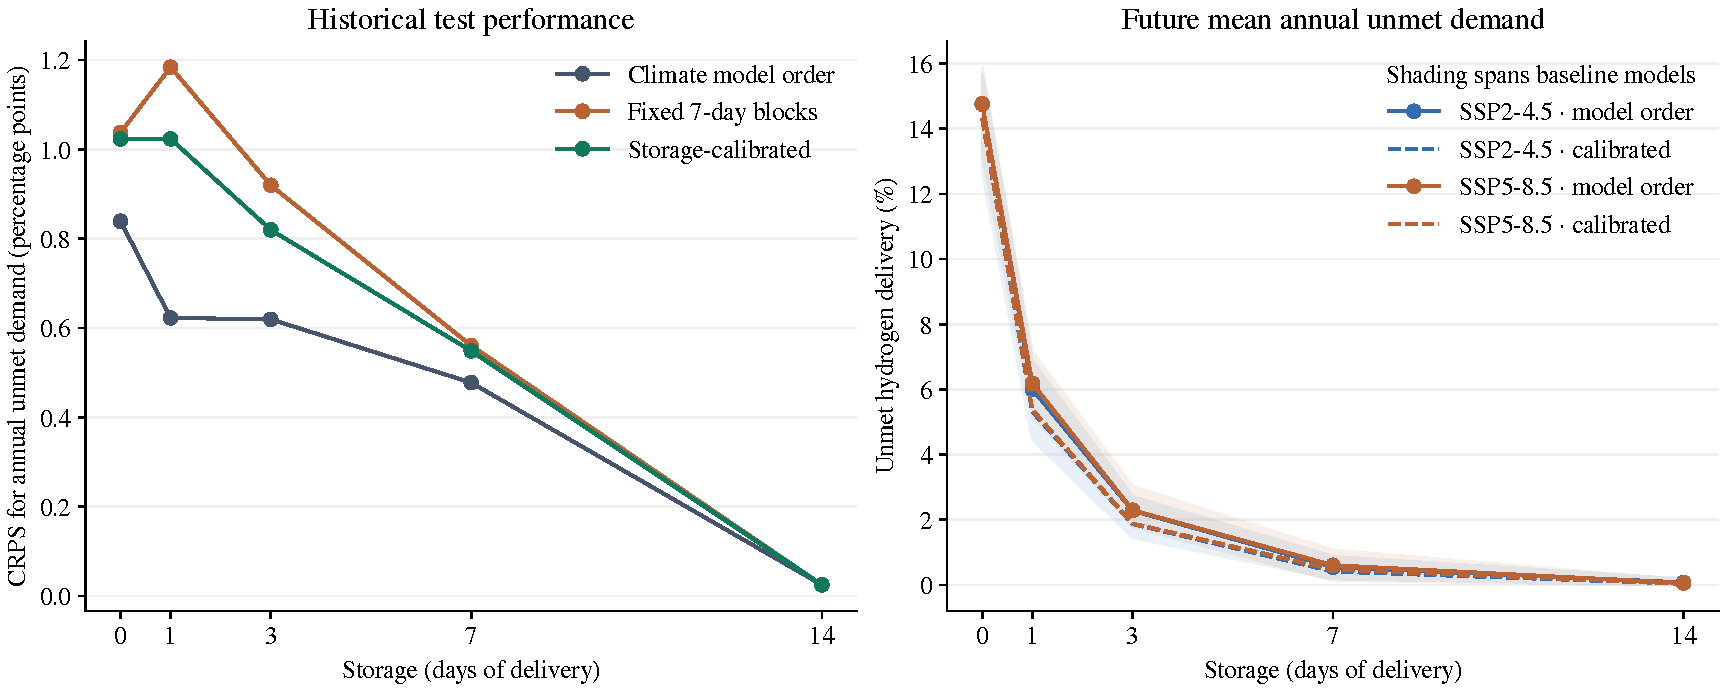
\includegraphics[width=\linewidth]{figures/hydrogen.pdf}
\caption{Historical test CRPS and projected mean annual unmet demand by tank size. The future panel shows 2041--2060 means. Solid lines retain climate-model order, dashed lines use storage-calibrated rank blocks, and shading spans the three baseline model means. Lower historical CRPS indicates better distributional agreement with the ERA5 reference.}
\label{fig:hydrogen}
\end{figure}

\clearpage
\begin{figure}[H]
\centering
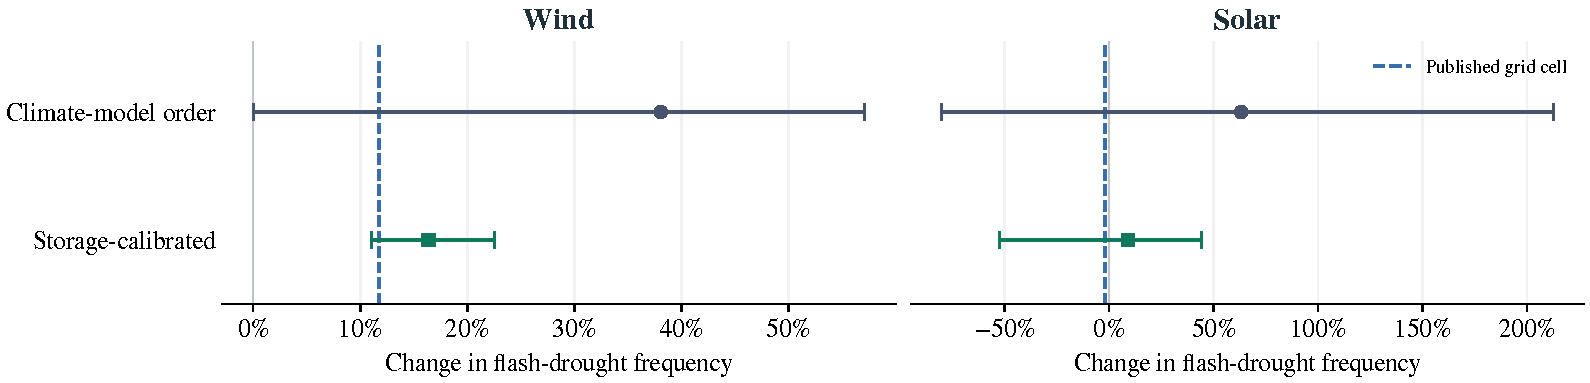
\includegraphics[width=.94\linewidth]{figures/flash-droughts.pdf}
\caption{Projected change in wind and solar flash-drought frequency under SSP2-4.5, comparing 2045--2074 with 1985--2014. Points show the pilot mean and horizontal intervals show the minimum and maximum across three models. The vertical marker in each panel shows the nearest eligible cell from the published Figure~2 workbook. The panels use separate horizontal scales.}
\label{fig:external}
\end{figure}

\section{Reproduction and data audit}
\label{app:reproduction}
The \RepoRoot\ provides the source, study configuration, and public-input retrieval code. To reproduce the experiment and the published-data comparison, use the benchmark branch, install the locked Python 3.12 dependencies and the workbook reader, then run the following commands from the repository root.

\begin{verbatim}
python -m beyond_normal.data all
python -m beyond_normal.run
python -m beyond_normal.benchmark --download
python -m beyond_normal.data cmip6 --future-years 2045 2074 \
  --experiments ssp245 --output data/raw/lin-2026
python -m beyond_normal.benchmark
python -m unittest discover -s tests -v
\end{verbatim}

The \RepoBenchmarks\ pin the results at commit \href{\RepoURL/commit/83839f69de4a26d76416b49299778d05279e79ef}{\texttt{83839f6}}. The \href{\RepoURL/blob/hydrogen-benchmarks/study.toml}{study configuration} records the plant, periods, scenario settings, and random seed. The \href{\RepoURL/blob/hydrogen-benchmarks/data/source/cmip6_stores.csv}{pinned CMIP6 catalog} records the exact realization, grid, version, and source URL. The \href{\RepoURL/blob/hydrogen-benchmarks/reports/run_manifest.json}{pipeline manifest} lists input and configuration checksums, software versions, and the selected parameters. The \href{\RepoURL/blob/hydrogen-benchmarks/reports/flash_drought_manifest.json}{external comparison manifest} specifies the grid cell, input periods, and checksum of the source workbook archive. The \href{\RepoURL/blob/hydrogen-benchmarks/reports/flash_drought_model_comparison.csv}{model-level counts} allow the published comparison to be audited before averaging.
